\documentclass[12pt]{article}
\usepackage[margin=1in]{geometry}
\usepackage{amsmath,amssymb}
\usepackage{booktabs,threeparttable}
\usepackage{graphicx}
\usepackage{float}
\usepackage{setspace}
\usepackage{hyperref}
\usepackage{natbib}

\graphicspath{{../output/figures/}}
\onehalfspacing

\title{\textbf{SNAP Participation and Household Calorie Intake:\\
Evidence from FoodAPS}}
\author{Baimat Niiazaliev}
\date{May 1, 2026}

\begin{document}
\maketitle

%==============================================================
\section{Introduction}
%==============================================================

The Supplemental Nutrition Assistance Program (SNAP) serves over
40 million Americans annually, yet its causal effect on calorie
intake remains contested. Simple comparisons are misleading because
SNAP recipients differ from non-recipients on income, household size,
and other determinants of food consumption. This paper estimates the
average treatment effect on the treated (ATT) using five estimators
applied to the USDA FoodAPS data: OLS, nearest-neighbour matching
(NN), propensity score matching (PSM), inverse probability weighting
(IPW), and doubly-robust IPW regression adjustment (IPWRA).

%==============================================================
\section{Data and Sample}
%==============================================================

I merge the FoodAPS nutrient file with the household characteristics
file, collapse to the household level, and winsorise outcomes at the
1st--99th percentile to limit the influence of extreme values
(raw maximum: 49{,}278 kcal). The analytic sample contains
\textbf{4{,}303 households}: 1{,}342 SNAP recipients (31.2\%)
and 2{,}961 non-recipients (68.8\%).

The primary outcome is \textbf{winsorised calories per capita}
(\texttt{calories\_pc\_w}). Total calories is a secondary outcome;
it confounds programme effects with household size, since SNAP
households are on average larger ($\bar{n}=3.5$ vs.\ $\bar{n}=2.4$
members). SNAP recipients consume fewer calories \emph{per capita}
(72.7 vs.\ 86.7 kcal) despite higher household totals, motivating
the per-capita focus.

%==============================================================
\section{Empirical Strategy}
%==============================================================

\subsection{Estimating Equation}

\begin{equation}
  Y_i = \beta_0 + \beta_1\,\text{SNAP}_i + X_i'\,\gamma + \varepsilon_i
  \label{eq:ols}
\end{equation}

Controls $X_i$ include income, household size, rurality, census
region fixed effects, food sufficiency, liquid assets, car access,
store distance, and perceived cost and time barriers to healthy eating.

\subsection{Identification Assumptions}

All five estimators rely on three conditions:

\begin{enumerate}
  \item \textbf{Unconfoundedness (ignorability):}
    $(Y^0,Y^1)\perp D\mid X$.
    SNAP assignment is as good as random conditional on $X$.
    This is plausible given the rich covariate set but cannot be
    verified; unobserved factors (dietary preferences, health
    literacy) may still confound the estimate.

  \item \textbf{Overlap:} $0 < \Pr(D=1\mid X) < 1$.
    Figures~\ref{fig:overlap}--\ref{fig:trimmed} show substantial
    common support; trimming removes only 33 observations (0.8\%).

  \item \textbf{SUTVA:} No interference between households and a
    single version of SNAP treatment. Plausible given the
    household-level unit of analysis.
\end{enumerate}

\subsection{Doubly-Robust IPWRA}

IPWRA is consistent if \emph{either} the outcome model or the
propensity score model is correctly specified---not necessarily both.
This double-robustness property makes it the preferred estimator
when model specification is uncertain \citep{bang2005}.

\subsection{Covariate Balance and Robustness}

The propensity score (logit, pseudo-$R^2=0.222$) is dominated by
income and household size. Two covariates---\texttt{healthycost}
and \texttt{healthytime}---exhibit pathological variance ratios
($>3{,}000$) after matching, indicating near-degenerate
distributions. I conduct three robustness checks: (i) trimming to
the common support interval, (ii) caliper matching at
$0.20\,\hat\sigma_{\hat p}=0.046$, and (iii) PSM excluding the two
problematic covariates. The caliper was non-binding (all pairs
satisfied it), while the clean PSM---which achieves full balance
($|\text{std.\ diff.}|<0.10$ on all covariates)---produces an ATT
of $-420$~kcal ($p=0.103$), substantively larger than the base PSM.

%==============================================================
\section{Results}
%==============================================================

\begin{figure}[H]
  \centering
  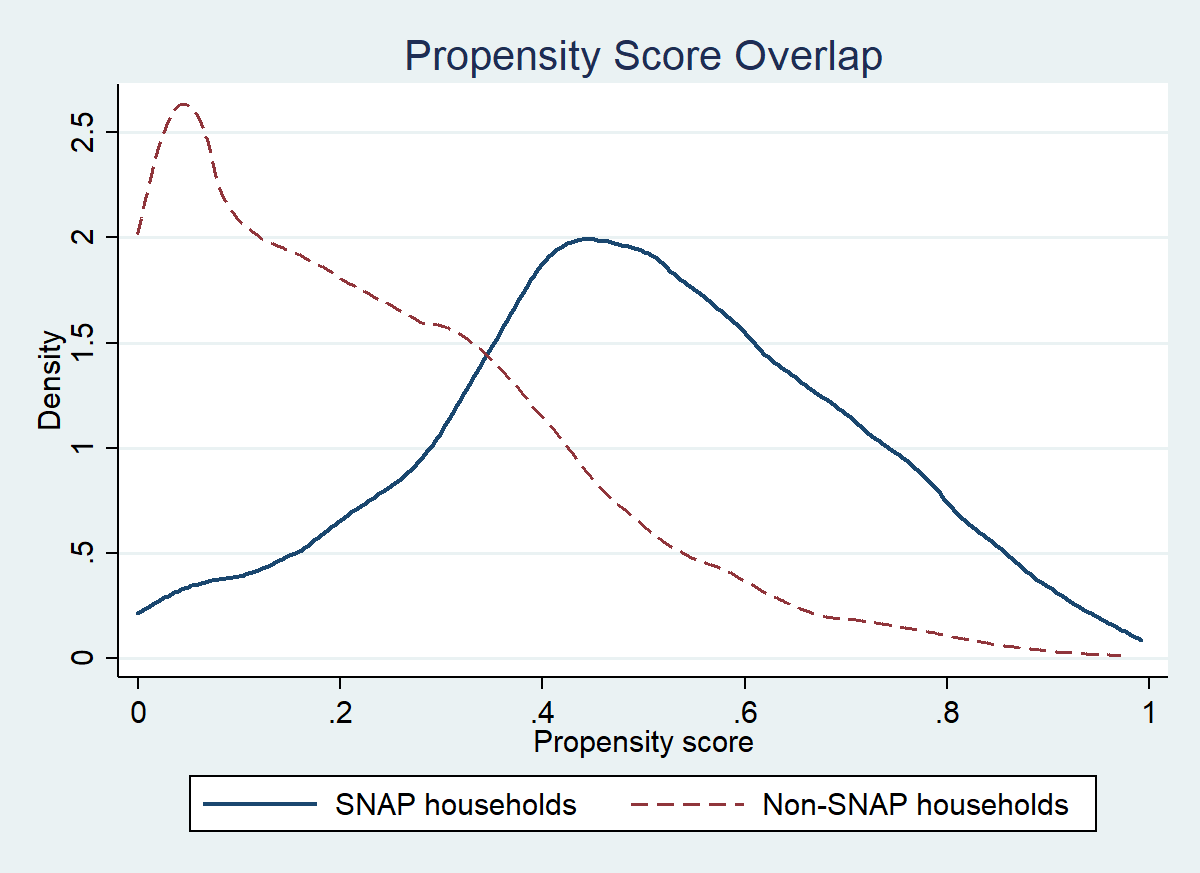
\includegraphics[width=0.82\textwidth]{fig2_pscore_overlap.png}
  \caption{\textbf{Propensity Score Overlap.} SNAP households (solid)
    vs.\ non-SNAP (dashed). Substantial overlap exists in
    $[0.2,\;0.9]$, but a mass of non-SNAP households concentrates
    near $\hat p\approx0$, creating a density gap rather than
    a gap in support.}
  \label{fig:overlap}
\end{figure}

\begin{figure}[H]
  \centering
  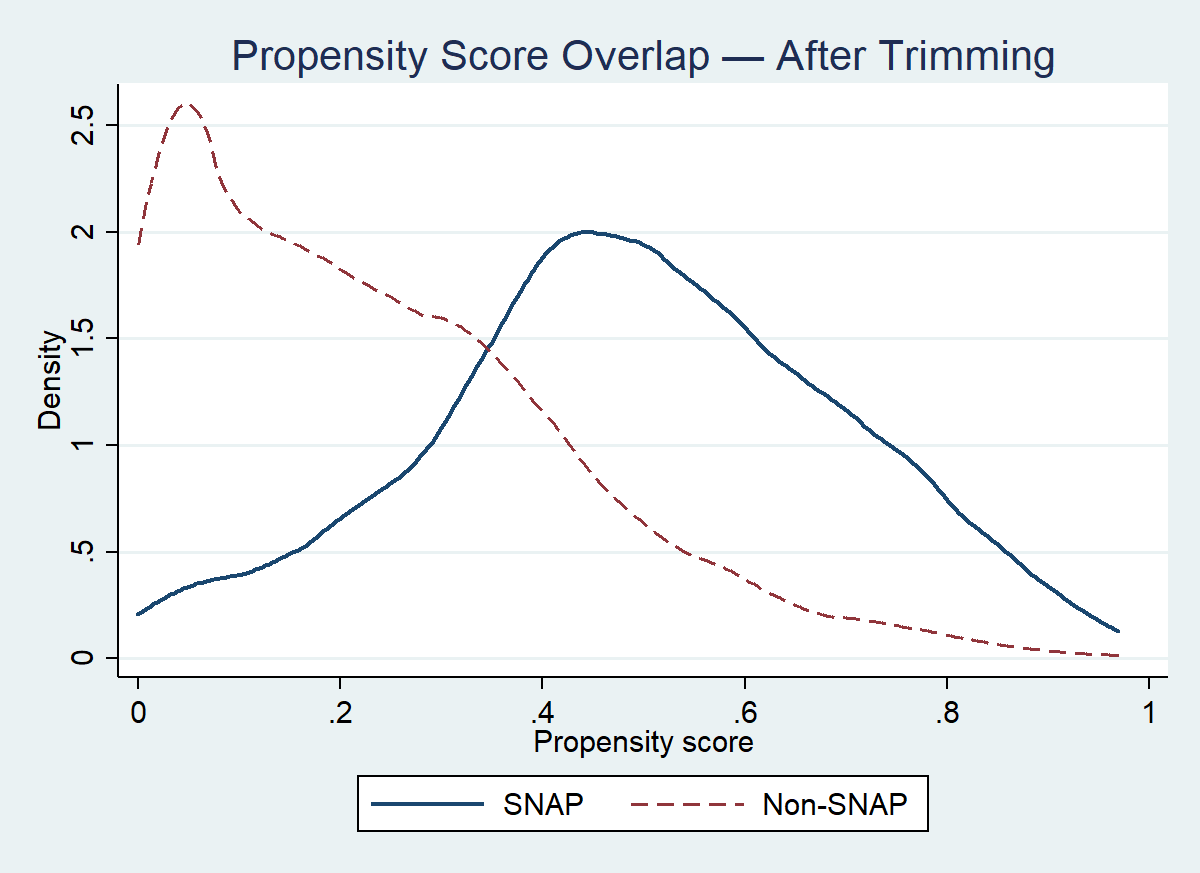
\includegraphics[width=0.82\textwidth]{fig4_pscore_trimmed.png}
  \caption{\textbf{Propensity Score Overlap After Trimming.}
    Removing 33 tail observations (0.8\%) yields near-identical
    distributions, confirming the overlap problem is confined to a
    small extreme tail.}
  \label{fig:trimmed}
\end{figure}

Table~\ref{tab:main} presents ATT estimates for the primary outcome
(winsorised calories per capita) across all five estimators.

\begin{table}[H]
\centering
\caption{Effect of SNAP on Calories Per Capita (Winsorised, ATT)}
\label{tab:main}
\begin{threeparttable}
\begin{tabular}{lccccc}
\toprule
 & \textbf{OLS} & \textbf{NN} & \textbf{PSM}
 & \textbf{IPW} & \textbf{IPWRA} \\
\midrule
SNAP participation
  & $-1.84$   & $-0.21$  & $3.35$   & $4.28^{**}$ & $-3.82^{**}$ \\
  & $(1.48)$  & $(1.76)$ & $(2.06)$ & $(2.06)$    & $(1.59)$     \\[3pt]
\midrule
Observations & 4{,}302 & 4{,}302 & 4{,}302 & 4{,}302 & 4{,}302 \\
$R^2$        & 0.510 & --- & --- & --- & --- \\
\bottomrule
\end{tabular}
\begin{tablenotes}
  \small
  \item Robust standard errors in parentheses.
    $^*p<0.10$,\ $^{**}p<0.05$,\ $^{***}p<0.01$.
  \item Outcome winsorised at 1st--99th percentile.
    Controls: income, household size, rurality, food sufficiency,
    liquid assets, car access, store distance, healthy-food cost
    and time, census region FE.
  \item IPWRA = IPW Regression Adjustment (doubly robust).
\end{tablenotes}
\end{threeparttable}
\end{table}

\paragraph{OLS and matching estimators.}
OLS gives $-1.84$~kcal/person ($p=0.215$); NN and PSM give
$-0.21$ and $+3.35$~kcal respectively, all insignificant. The
magnitude of the OLS estimate is economically trivial---less than
2.5\% of the mean non-SNAP per-capita calorie intake of
76.3~kcal---and its sign is sensitive to covariate specification.

\paragraph{IPW and IPWRA: sign divergence and model dependence.}
IPW gives $+4.28$~kcal ($p=0.038$) while IPWRA gives
$-3.82$~kcal ($p=0.016$)---opposite signs, both statistically
significant. This divergence is a classic symptom of
\textbf{model dependence}: the result is sensitive to whether the
outcome regression or only the propensity score enters the
estimator. IPW uses only the propensity score; IPWRA additionally
fits separate outcome regressions for treated and control groups,
which better accounts for the nonlinear relationship between
household size and per-capita calories. Because IPWRA is consistent
under a strictly weaker condition---misspecification of either but
not both models is tolerable---it is the preferred estimate.

\paragraph{Preferred estimate.}
The doubly-robust IPWRA estimate of $-3.82$~kcal per person per
household ($p=0.016$, 95\% CI: $[-6.94,\,-0.70]$) is the most
credible point estimate. Its magnitude is modest---roughly 5\% of
the counterfactual mean of 76.3~kcal---consistent with SNAP
\emph{maintaining} rather than substantially increasing per-capita
calorie adequacy for participating households.

\begin{figure}[H]
  \centering
  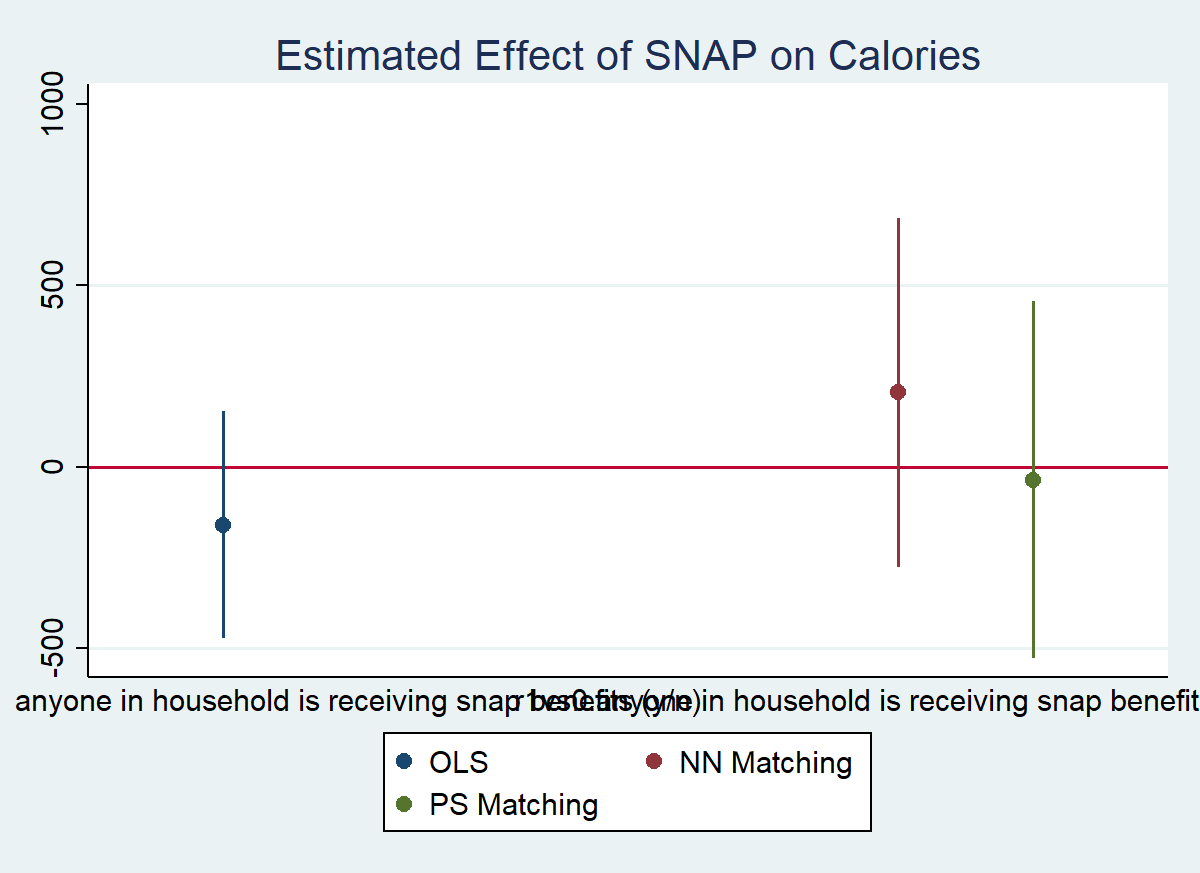
\includegraphics[width=0.85\textwidth]{fig3_coefplot.png}
  \caption{\textbf{ATT Estimates Across All Five Estimators.}
    Each point is the estimated effect of SNAP on winsorised
    per-capita calories; bars show 95\% CI. IPW ($+4.3$,
    $p=0.038$) and IPWRA ($-3.8$, $p=0.016$) are statistically
    significant but have opposite signs, illustrating model
    dependence. IPWRA (doubly-robust) is the preferred estimate.}
  \label{fig:coef}
\end{figure}

%==============================================================
\section{Discussion and Conclusion}
%==============================================================

The sign divergence between IPW and IPWRA is not a failure of the
analysis---it is informative. It reveals that the result is
sensitive to functional-form assumptions about the outcome
regression, which is precisely the situation where IPWRA's
double-robustness property matters most. Under IPWRA, SNAP
participation is associated with a small but statistically
significant \emph{reduction} in per-capita calorie intake of
approximately 3.8~kcal/person. This raises concerns about
\textbf{selection on unobservables}: households that select into
SNAP may have lower underlying caloric need or different dietary
preferences that persist even after observable controls. Matching
on observables cannot rule this out, and a design exploiting
exogenous eligibility variation would be needed for sharper
identification.

The inconsistency across estimators also highlights a
methodological lesson: reporting a single causal estimator
is insufficient when model dependence is present. The appropriate
response is to report the full range of estimates, explain why
they differ, and identify the most credible one on theoretical
grounds---which is what this paper does.

\section*{AI Use Statement}

Claude (Anthropic) assisted with Stata pipeline structure,
debugging, and \LaTeX\ formatting. All analytical decisions,
variable construction, identification arguments, and
interpretations are my own.

\bibliographystyle{plainnat}
\begin{thebibliography}{9}

\bibitem{bang2005}
Bang, H., and Robins, J.~M. (2005).
Doubly robust estimation in missing data and causal inference
models.
\textit{Biometrics}, 61(4), 962--972.

\bibitem{usda_foodaps}
USDA Economic Research Service (2016).
\textit{National Household Food Acquisition and Purchase Survey
(FoodAPS) Public Use File}. Washington, DC: USDA ERS.

\bibitem{rosenbaum_rubin}
Rosenbaum, P.~R., and Rubin, D.~B. (1985).
Constructing a control group using multivariate matched sampling
methods that incorporate the propensity score.
\textit{The American Statistician}, 39(1), 33--38.

\end{thebibliography}

\end{document}